\section{Application of AllocMinDistLocalSearch to Geomarketing strategies}
The aim of this thesis is the comparison of different approaches for area segmentation process to define the most promising one for application to Geomarketing strategies. Therefore different approaches were developed and implemented so that a comparison was possible. The comparison shows that the approach called AllocMinDistLocalSearch yields the best results concerning the requirements from the field of Geomarketing. During the AllocMinDistLocalSearch algorithm first basic areas are allocated to territory centres dependent on their distance to the centres. Afterwards in second step the basic areas are rearranged again to get balanced territories concerning an activity measure. The implementations have shown that there some improvements are necessary to make AllocMinDistLocalSearch applicable for Geomarketing strategies. These ones will be considered during the application and will be explained in more detail within the following sections. The algorithm will be applied to three defined kinds of strategies. One type will be the area segmentation itself which is applied during political distriction and by the optimization of existing sales districts for instance. Within these analyses already fixed territory centres are available. The second Geomarketing strategy is called Greenfield analysis. This one owns no given territory centres. Consequently at first some centres need to be defined. Afterwards the area segmentation algorithm can be applied. Whitespot analyses are a combination of area segmentation and Greenfield analyses. Within the Whitespot analyses already some territory centres exists. Additionally to the existing ones, new centres need to be created. To all these centres (given ones and new ones) the area segmentation of the basic areas will be done. All three kinds of analyses will be explained in more detail within the following sections. 


\subsection{Area segmentation and optimization}\label{areaseg}
The area segmentation process is the main approach an can be found in both other used type of strategies too. Consequently this algorithm needs to be dependable and need to provide satisfying results because it affects the solution of the others too. Area segmentation processes are the core of all applied districtions for example political distriction, sales distriction and the optimization of sale territories. With the help of area segmentation processes a clustering of basic areas will be done into a predefined number of territories. Thereby one or more specific activity measures need to be considered. Within the case study just household numbers are considered during the allocation. During the comparison of different approaches it was determined that AllocMinDistLocalSearch yields to the best results. But the algorithm offers some weaknesses yet consequently enhancements are necessary to implement. Therefore the main ideas of AllocMinDistLocalSearch are taken. The process will be amplified by checking some constraints to satisfying the requirements from the field of Geomarketing. The most important constraint is the location of the territory centres within the territories which belong to it. Therefore it will be determined which basic area contains the territory centre. The resulting basic areas will be saved and considered all the time during the allocation. Remembering the structure of AllocMinDistLocalSearch it was recognizable that it consists of two steps. In first step basic areas are allocated to the territory centres dependent on their distance. In second step local search will be applied to realize the balance constraint. Within the first step the centre is always located within the territory even if the constraint is not applied. The problem of residing outside exists first during the rearrangement. Consequently before a basic area will be rearranged it will be checked whether it is the saved basic area, which contains the territory centre. If this is the case, the basic area will not be rearranged. Thus another basic area needs to be chosen. That means the basic areas containing the centres are preserved all the time for rearranging. \\
Besides the location of the territory centres, it will be postulated that the created territories need to be contiguous. For satisfying the coherence two different steps are need to implemented. The first step will be applied to the AllocMinDist approach which is used in first step of AllocMinDistLocalSearch. In most of the cases the created territories are coherent and compact after that step. But this result is not given all the time. Sometimes some basic areas are allocated in such a way that no contiguity within a territory exists. This problem was already mentioned during the analysis of the implementation of AllocMinDist. Consequently a check needs to be done after the first step of AllocMinDistLocalSearch to satisfying the coherence of the territories. Therefore each created territory will be checked whether all basic areas are contiguous. If this is the case, the next territory will be taken. If the check concludes with an incoherency basic areas will be rearranged to another territory. Therefore the part which is located apart will be defined. For doing so all basic areas of the territory are taken. From the amount of areas firstly the area is chosen which contains the territory centre. Afterwards all basic areas are determined which can be reached from that area using a graph. All basic areas which are not linked to the amount of basic areas that are reachable are the ones which need to be rearranged. Figure 36 illustrates the graph on an example.

\begin{figure}[H]
	\centering
	\includegraphics[width=1\textwidth]{images/graphwhitepic.jpg}
	\caption[Using a graph for determining incoherence]{Using a graph for determining incoherence. All basic areas that can be reached by an edge of the graph (black lines linked by nodes) are contigous. Thus, one basic area needs to be rearranged. Example territory using zip-code8 areas.}
\end{figure}

After the check all territories are contiguous so that a satisfying base exists for doing the rearrangement by local search. Previously all neighbouring territories are determined to define the one with the highest sum of activity measure. This territory has to deliver one basic area to the territory with the smallest sum of activity measure. Doing so maybe a basic area is given that causes an incoherency in one of the two areas for instance by diving the territory that gives the area into two half's. Consequently a check is necessary again whether the basic area can be given. Therefore the same approach is used like after step one. By comparing the resulting graphs of both territories it can be determined whether both ones are contiguous anymore after change. If the contiguity is given for both territories the change can be done. For creating the graph knowledge about neighbouring relationship need to be there. Two basic areas are neighboured if they are sharing edges or points. Determining the neighbour relationships can be done with the help of a function in PostGIS which determines all neighbours of a geometry. These information can be saved and used during the creation of the graph. Thus no additional access to the database is necessary. Another possibility is checking the coherency with the help of a PostGIS function. But this approach needs a lot of additionally database access consequently the run time raises much. Thus this approach was abandoned by performance issues. \\
Additionally to contiguity the compactness of the territories is important. For evaluating the quality of compactness the measure of Cox is used. During the evaluation of the algorithms the compactness measure was just applied afterwards for determining the quality of compactness. Instead of this the measurement will be applied during the rearrangement to get more compact territories. Therefore the compactness of the territories need to be initialized after doing the first arrangement by AllocMinDist in first step. With the help of the initial values of compactness the rearrangement can be done in such a way that the compactness will be considered. Caused by the balance constraint it can be happen that basic areas need to be allocated in such a way that the compactness getting worse. Consequently a solution needs to be implemented to weight both constraints. Therefore a function was created which includes both constraints: compactness and balance. The function measures the changes of compactness and balance concerning both values before and after rearranging. The resulting values show whether the rearrangement produces a better resolution or not. Consequently all possible basic areas that may be rearranged can be checked so that the one can be chosen that provides the best result. Let $\Delta \phi $ denotes the changes of compactness and balance it can be written as

\[ \mathit{\Delta \phi = \phi_{new}-\phi_{old} \to min}\]

$\phi_{new}$ and $\phi_{old}$ need to be calculated using the alteration of balance and compactness including weighting values. The resulting value of $\Delta \phi$ may be smaller or greater 0. If the value is smaller 0, the arrangement yields to a better resolution than before the rearrangement. Vice versa a value greater 0 denotes a degeneration. Consequently the value needs to be as minimal as possible. 
Let $w$ denotes the weightings, $\Delta c$ denotes the change of compactness and $\Delta b$ denotes the change of the balance value thus the calculation of $\phi$ can be formulated as

\[ \mathit{\phi = \Delta c * w_{1} + \Delta b * w_{2} \to min}\]

$\Delta c$ will be calculated using the compactness measure of Cox. The resulting value will be normalized by 

\[ \mathit{\Delta c = 1 - c \to min}\]

The same will be done during the calculation of the change of balance value. For calculating the balance value the difference to the given sum of activity measure will be used that each territory should contain. That difference is normalized similar to the compactness measure.

\[ \mathit{\Delta b = 1 - b \to min}\]

The normalizing is necessary for the application of the weighting values. The weighting values can be defined by the user and need to be values between 0 and 1. The application of the algorithm using the weighting function shows that the weighting needs to be determined in benefit of balance if the threshold value is defined to be small. The threshold value is used for defining the allowed difference of the sum of activity measure comparing the territories. At the same time case studies show that a weighting for the benefit of balance does not mean automatically that worse balanced territories will be achieved. The weighting value just determines which basic areas will be preferred during the rearrangement. \\ 
The algorithm for area segmentation processes was applied to the same test data which were used during the implementation and comparison of different heuristic approaches. The results of different test cases using several weighting values and thresholds are shown in Figure 37.

\begin{figure}[H]
	\centering
	\includegraphics[width=1\textwidth]{images/areasegmentation.jpg}
	\caption[Application of area segmentation algorithm to zip-code5 and zip-code8 areas.]{Application of area segmentation algorithm to zip-code5 and zip-code8 areas. a) Weighting values: compactness 1, balance 0, threshold 50. b) Weighting values: compactness 0, balance 1, threshold 30. c) Weighting values: compactness 1, balance 0, threshold 50. a) Weighting values: compactnes 1, balance 0, threshold 100}
\end{figure}

The results show that the resolution achieved by the area segmentation process depends on the chosen values for the weighting and the threshold. By using the compactness measure the territories are more compact. Their shapes were confirmed by some Geomarketing specialist which have considered them as compact. During the calculation of the compactness measure the areas and circumferences of the territories are used. These ones can be calculated with the help of functions provided by PostGIS. Performance tests showed that these calculations need a lot of time because they are done several times during the rearrangement. Consequently a solution was implemented which uses no access to the database. Instead of this the areas, circumferences and shared edges of basic areas were saved at the beginning. Thus only one time a database access was necessarily. Afterwards every calculation can be done with the help of the stored information. \\
The rearrangement of basic areas during the local search offer some problems. It can be recognized in some cases that the predefined threshold value will be not reached because always the same basic areas are rearranged again and again so that no correction of the sum of activity measure will be achieved. Several approaches were tried to find a solution for this problem but no optimal one could be found. Within AllocMinDistLocalSearch the territory with smallest sum of activity measure was determined. This one took a basic area from the territory with biggest sum of activity measure. Test have shown that the problem of endless rearranging occurs more often in such approach than using the approach which is implemented now. Now the sum of all territories are checked whether the threshold value of balance is satisfied. If one territories does not fulfill the threshold value a basic area will be rearranged. If a territory satisfy the value nothing happens and thus the next territory will be checked. As soon as all territories satisfying the threshold value the algorithm ends. Caused by the endless rearrangement a break needs to be implemented to get a solution in the end. Although other approaches were tried too for optimizing the rearrangement process the implemented one yields to the best results. Nevertheless improvements are necessary to get satisfying results all the time. The workflow diagram of the implemented algorithm can be found in Figure 38. 

\begin{figurevarSize}{Workflow diagram of implemnted area segmentation approach}{images/areasegmentation_workflow.jpg}{0.85}\end{figurevarSize}

The initialization process consists of several sub process. Besides the geometries also the neighbours need to be initialized. Additionally centroids of each basic area are calculated used for determining the distances between territory centres by using orthodroms. Furthermore areas and circumferences are saved to use them during the rearrangement.

\begin{figurevarSize}{Processes of the initialisation}{images/init.jpg}{0.25}\end{figurevarSize}

\subsection{Greenfield  analysis}

Greenfield analyses are a special type of strategies for planning new locations. When a company will be founded at the beginning no branch exists. Consequently it may be needed to determine possible places for locations so that a meaningful area segmentation considering an activity measure can be done. Besides the planning of new locations for a company also political distriction using no predefined centres is an example of an approach similar to the Greenfield analyses. Doing the analysis it is first necessary to determine possible locations before the area segmentation can be done. Consequently an algorithm is needed which consists of two steps similar to location-allocation approaches. For defining possible places for the locations an approach similar to EatUpMinDist will be used. The comparison of the algorithms showed that this approach is not usable using fixed centres. But doing Greenfield analysis in the beginning no centres exists consequently the approach may be promising. The EatUpMinDist algorithm needs to be adapted in such a way that a meaningful starting point can be determined. Therefore a basic area resides on the outer border of the investigation area, will be chosen. Starting from that chosen area the first territory will be grew up at the boundary of the territory by allocating basic areas until a threshold value is reached. The threshold value is calculated by summing the activity measures of all basic areas and dividing them through the number of territories that will be created. For generating the next territory the next basic area at the boundary will be chosen which is not allocated yet. Doing so the condition needs to be satisfied that the basic area is neighboured by the territory that was created before. As soon as a basic area was found the territory can be created. This will be done until the predefined number of territories is reached. If no basic area at the boundary exist anymore, another basic area is chosen which is neighboured by the territory created before independently on the location of that area. If no not yet allocated basic area, which is neighboured by the territory, is available anymore a basic area will be taken which is not neighboured but yet not allocated. Following these steps all territories can be created. Figure 40 shows the created territories after the first step using the case study investigation area.

\begin{figurevarSize}{Created intial territories for defining initial territory centres during a Greenfield analysis}{images/greenfieldfirst.jpg}{0.7}\end{figurevarSize}


The problem using this approach is given by the threshold value to abort the allocation of basic areas to one territory. It was already mentioned during the explanation of Eat-up and EatUpMinDist. By exceeding the threshold value for abortion it may happen that already all basic areas are allocated before the predefined number of territories is reached. To prohibit this phenomena additionally abortion criteria need to be defined to ensure that all territories contain at least one basic area. This can be done by checking the resulting number of not yet allocated basic areas. \\
After the creation of initial territories is done territory centres can be determined by setting the centres into the middle of each territory. Afterwards these centres can be used doing the area segmentation. The used  algorithm is the same which is used in section \ref{areaseg} ''\hyperref[areaseg]{Area segmentation and optimization}''. This one will be applied using the predefined territory centres. As soon as the area segmentation is passed final territory centres will be determined. The following figures show the workflow and results of that calculation using different values for weighting and threshold. In both application 10 territories and thus 10 locations are created.

\begin{figurevarSize}{Workflow of algorithm used for Greenfield analysis}{images/greenfield_workflow.jpg}{0.3}\end{figurevarSize}

\begin{figure}[H]
	\centering
	\includegraphics[width=1\textwidth]{images/greenfieldend.jpg}
	\caption[Results of Greenfield analyses. ]{Results of Greenfield analyses. a) Zip-code5 areas. Weighting values: compactness 1, balance 0, threshold 50. b) Zip-code8 areas. Weighting values: compactness 0.1, balance 0.9, threshold 50.}
\end{figure}

Although the results of that case study look promising such resolutions are not satisfied all the time. Using other parameters or investigation areas the area segmentation process may be yield to worse results. Some possibilities are no well balanced territories or have a corrupted compactness. The origin of this can be the following two reasons: First, one problem is caused by the determination of the initial locations. They may be located in such a way that no area segmentation containing a satisfying result may be done. Second, the problems of the used area segmentation algorithm which are already mentioned in section \ref{areaseg}, also take an influence of the results here. Consequently it can be concluded, that the Greenfield algorithm yields to results but another solution which will be more robust may be necessary. Some additional test cases using several investigation areas and parameters may confirm or disprove that.

\subsection{Whitespot analysis}

Whitespot anaylses are a combination of area segmentation processes and Greenfield analyses. But instead starting on a greenfield the white spots between existing locations need to be determined to define places where new locations can be set. Consequently several numbers of locations are given at the beginning of the calculation. Additionally to these ones a predefined number of new locations will be set. In reality, mostly 1 up to 3 new locations will be created. All locations (given one and new created one) will be used during the application of the area segmentation. Consequently it is at first necessary to define the white spot for placing new locations. Afterwards the area segmentation process can be done using all locations. The implementation of the Whitespot analysis consists of three main steps:

\begin{enumerate}
	\item Creation of territories for given locations
	\item Creation of territories containing new locations so that initial new locations can be determined
	\item Application of area segmentation to given and initial locations
\end{enumerate}

As soon as the area segmentation process is done the final positions of the new locations can be determined. Considering the first two steps in more detail it can be recognized that an approach similar to EatupMinDist will be applied. At first for each given location the territories are created using EatupMinDist. The threshold value for aborting the allocation is calculated by the sum of of the activity measure of all basic areas divided by the sum of given and new locations.

\begin{figure}[H]
	\centering
	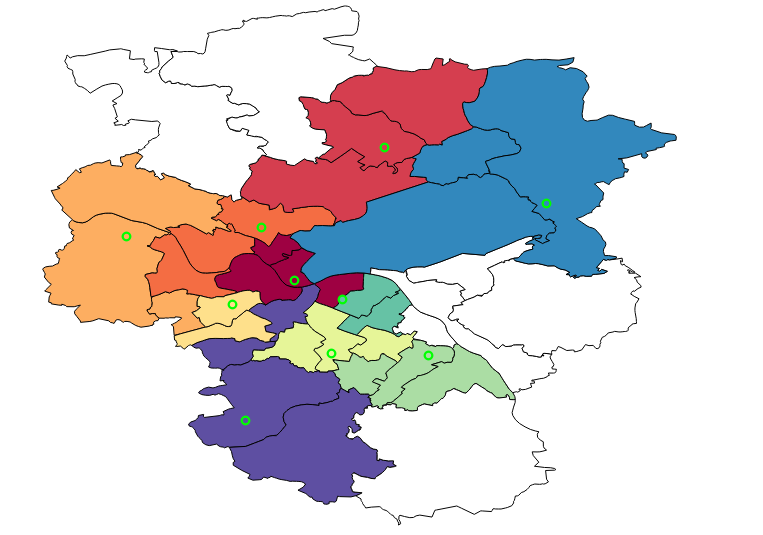
\includegraphics[width=0.5\textwidth]{images/1_allocationToGivenLocations.png}
	\caption{Allocation of basic areas to given locations within a Whitespot analysis}
\end{figure}

Afterwards the places of new locations need to be determined. In order to place the new locations, it is necessary first to necessary to define a starting point for creating the territory. Therefore three different approaches were implemented and compared determining the one which yields to best results. First approach uses the not yet allocated basic areas by their identification number. All number will be ordered and the one with smallest ID will be taken. Consequently no consideration of location of the basic area or value of activity measure are done during the determination of the starting point for new locations. The second algorithm uses just basic areas that are located at the boundary of the investigation area. These basic areas are ordered by their IDs and again the one with the smallest number is taken. That approach considers the location of basic areas after all but do not consider any activity measure. That is why the third approach was developed. That one considers all basic areas that are not allocated yet. Thereby all basic areas from that amount which are contiguous will be respected as a territory. Afterwards the sum of the basic areas will be calculated for each possible territory. The one with the highest sum will be taken. Within that taken territory the basic area with highest activity measure is determined. This one is used as starting point. Considering the figure above this process will be explained using the figure as example. The figure shows that seven basic areas are not allocated yet. Using these areas three contiguous territories can be created. One territory contains two basic areas, the second one contains four areas and the last one comprises just one basic area. For each territory the sum of activity measure will be calculated. In the case of the example it will be determined that the territory containing four not yet allocated basic areas owns the highest value of activity measure. Consequently one basic area from that territory will be taken as starting point. Using a basic area as starting point a territory can be created using the same approach like EatUpMinDist uses. This process is equal within all three approaches. The allocation ends as soon as the threshold value is reached or no basic areas are allocatable anymore. It is not possible to allocate basic areas either if all basic areas are allocated or if no basic area exists that is coherent to the created territory. After the allocation to the territory is done the new location can be set into the middle of the area. Figure 44 shows the resolution of creating a new location using the third approach. The given locations are marked by green points, the new one is marked by a pink circle.

\begin{figure}[H]
	\centering
	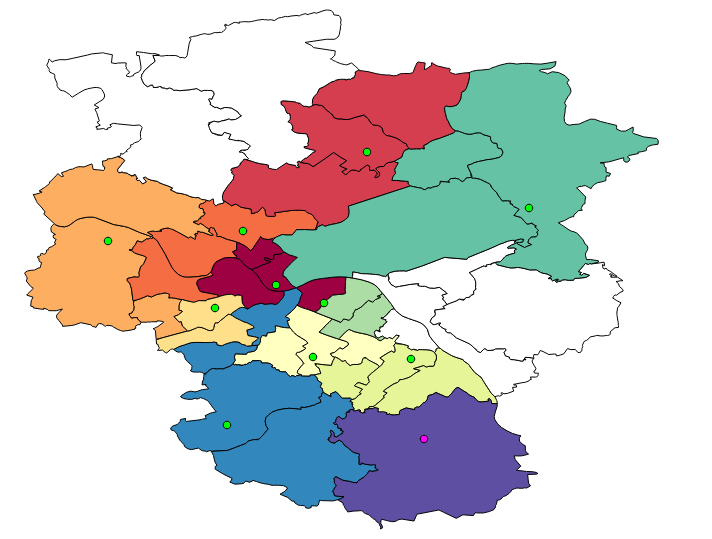
\includegraphics[width=0.5\textwidth]{images/2_allocationToGivenAndNewWithoutCheck.png}
	\caption{Result after creating a new territory containing the new location within a Whitespot analysis}
\end{figure}

The implementation of all three approaches showed that the third approach yields to the best results. Additionally it considers the locations and activity measures of basic areas so that it can be seen as the most advisable approach. Thus that one will be used for the Whitespot analyses. The figure shows that after creating territories for ten given and one new location, already some basic areas are not assigned yet. Consequently a check was implemented to allocate the resulting areas to existing territories. Afterwards the given and the new locations are used doing the area segmentation process. This one uses similar to Greenfield analyses the area segmentation algorithm from section \ref{areaseg} ''\hyperref[areaseg]{Area segmentation and optimization}''.\\
Within the following figures workflow and results using different calculation parameters are shown.

\begin{figurevarSize}{Workflow of algorithm used for Whitespot analysis}{images/whitespot_workflow.jpg}{0.9}\end{figurevarSize}

\begin{figure}[H]
	\centering
	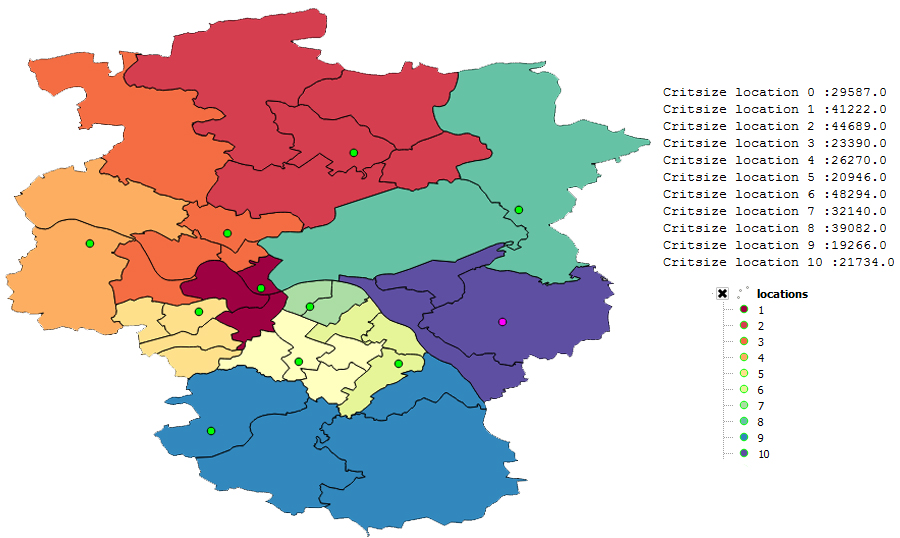
\includegraphics[width=1\textwidth]{images/whitespot.jpg}
	\caption[Results of Whitespot analyses using 10 given locations (green circle) and creating 1 new location (pink circle).]{Results of Whitespot analyses using 10 given locations (green circle) and creating 1 new location (pink circle). a) zip-code5 areas. a) zip-code8 areas.}
\end{figure}

The outcome of Whitespot analysis show results that are quite good. The created territories are contiguous as well as balanced. By implementing three different approaches determining the starting point during the creation of new locations the best one could be chosen and used. Consequently the created territories containing new locations are located quite well. Although the results look good some problems exist which are caused by the mentioned weaknesses of the area segmentation approach. By using that process also for Whitespot analyses they take influence to these results, too. Nevertheless the implemented algorithm is a usable approach for doing Whitespot analyses.